\section{Modelo conceptual del Proyecto}
\subsection{Descripción general}
 En la figura~\ref{fig:modeloConceptualProyectos} se muestra la estructura de información que manejará el sistema para registrar proyectos 
 y los colaboradores de la organización.
 
\begin{figure}[htbp!]
	\begin{center}
		\fbox{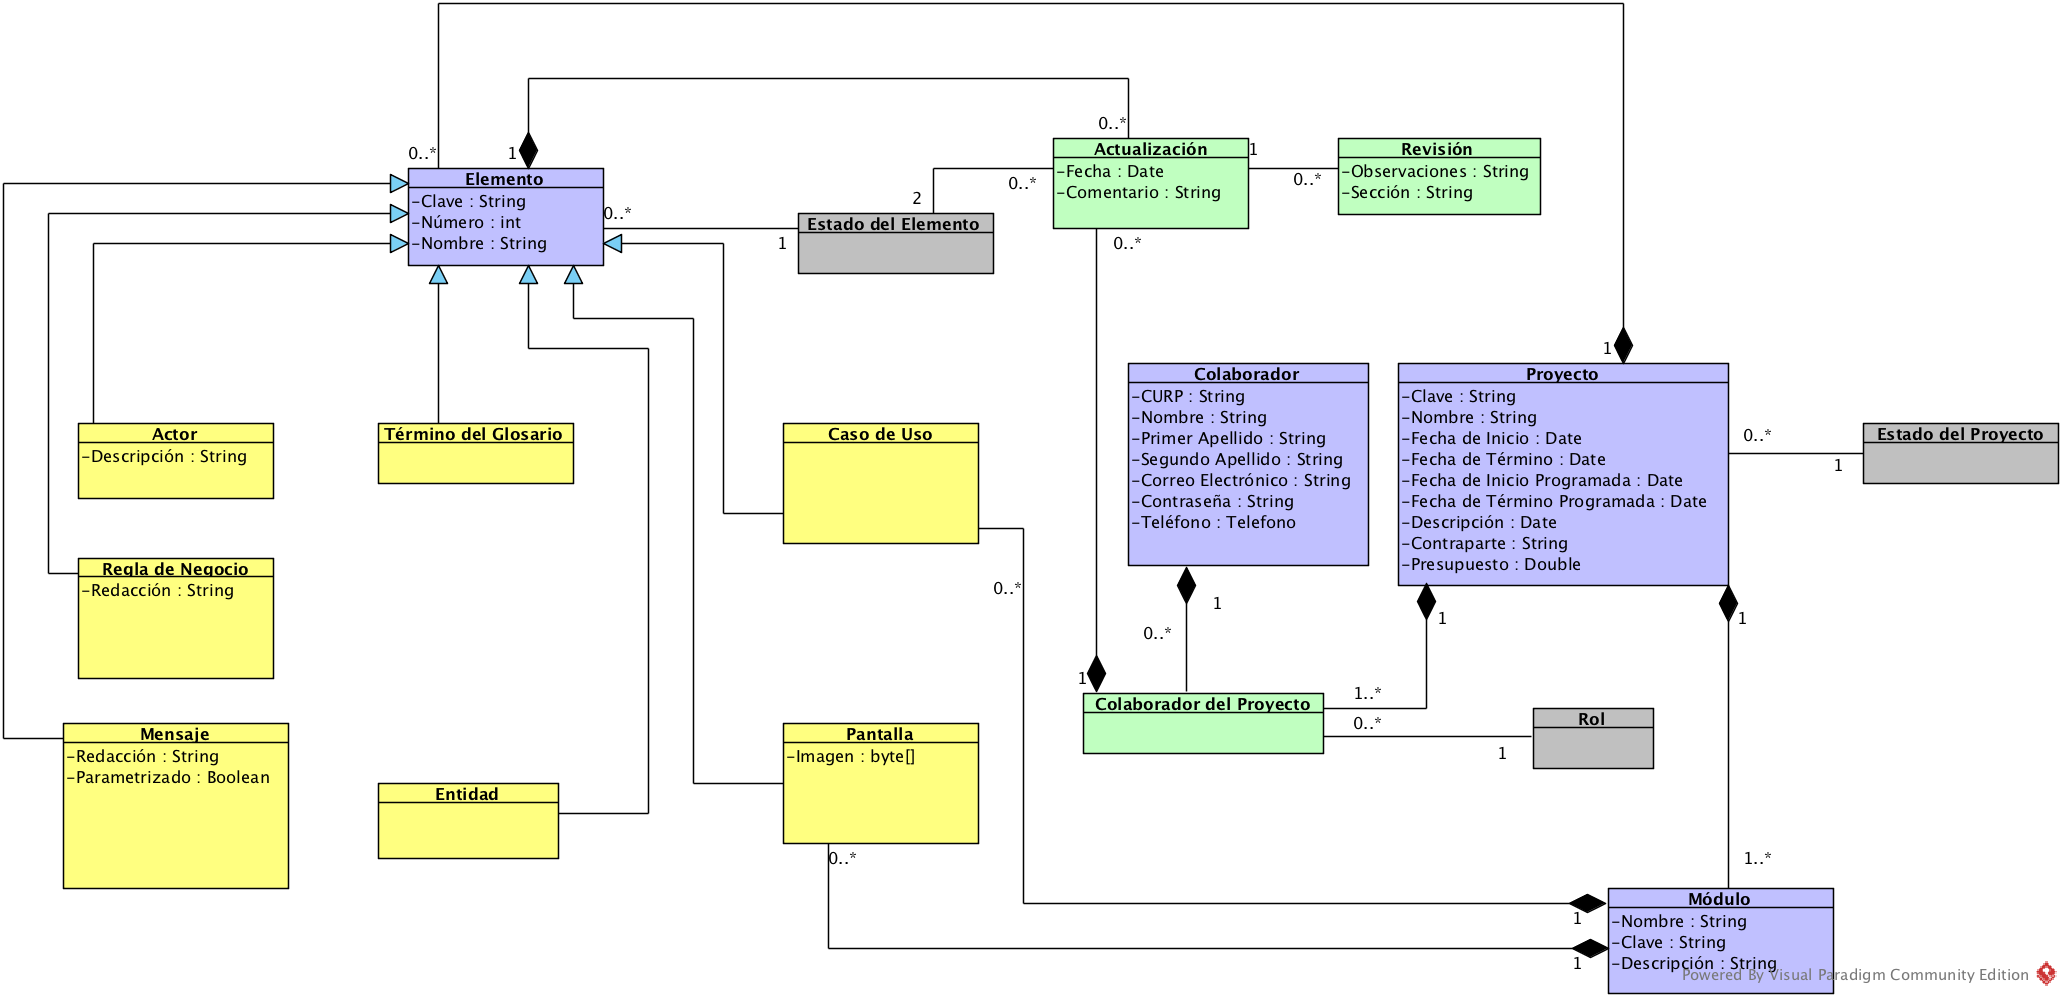
\includegraphics[width=1\textwidth]{ModeloNegocios/images/ModeloConceptualProyecto}}
		\caption{Modelo conceptual de proyectos}
		\label{fig:modeloConceptualProyectos}
	\end{center}
\end{figure}


%-------------------------------------------------Elemento----------------------------------
\begin{BusinessEntity}{Elemento}{Elemento}
      \Battr{Clave}{Clave}{\tdPalabra}{Clave que permitirá distinguir el tipo de Elemento}{\requerido}
      \Battr{Numero}{Número}{\tdNumerico{entero}}{Número del Elemento del tipo definido por la Clave}{\requerido}
      \Battr{Nombre}{Nombre}{\tdFrase}{Nombre que identificará al Elemento}{\requerido}
\end{BusinessEntity}

\subsubsection{Relaciones}

\begin{BusinessFact}{Elemento:Pantalla}{Pantalla}
	\BRitem{Descripción}{Pantalla es un tipo de \cdtRef{elemento}{Elemento}.}
	\BRitem{Tipo}{\relHerencia}
\end{BusinessFact}

\begin{BusinessFact}{Elemento:RegladeNegocio}{Regla de Negocio}
	\BRitem{Descripción}{Regla de Negocio es un tipo de \cdtRef{elemento}{Elemento}.}
	\BRitem{Tipo}{\relHerencia}
\end{BusinessFact}

\begin{BusinessFact}{Elemento:Actor}{Actor}
	\BRitem{Descripción}{Actor es un tipo de \cdtRef{elemento}{Elemento}.}
	\BRitem{Tipo}{\relHerencia}
\end{BusinessFact}

\begin{BusinessFact}{Elemento:Mensaje}{Mensaje}
	\BRitem{Descripción}{Mensaje es un tipo de \cdtRef{elemento}{Elemento}.}
	\BRitem{Tipo}{\relHerencia}
\end{BusinessFact}

\begin{BusinessFact}{Elemento:Termino(Glosario)}{Término (Glosario)}
	\BRitem{Descripción}{Término (Glosario) es un tipo de \cdtRef{elemento}{Elemento}.}
	\BRitem{Tipo}{\relHerencia}
\end{BusinessFact}

\begin{BusinessFact}{Elemento:Entidad}{Entidad}
	\BRitem{Descripción}{Entidad es un tipo de \cdtRef{elemento}{Elemento}.}
	\BRitem{Tipo}{\relHerencia}
\end{BusinessFact}

\begin{BusinessFact}{Elemento:CasodeUso}{Caso de Uso}
	\BRitem{Descripción}{Caso de Uso es un tipo de \cdtRef{elemento}{Elemento}.}
	\BRitem{Tipo}{\relHerencia}
\end{BusinessFact}

\begin{BusinessFact}{Elemento:Actualizacion}{Actualización}
	\BRitem{Descripción}{Un elemento ha pasado por un conjunto de actualizaciones.}
      \BRitem{Tipo}{\relComposicion}
      \BRitem{Cardinalidad}{Uno a muchos}
\end{BusinessFact}

\begin{BusinessFact}{Elemento:EstadodelElemento}{Estado del Elemento}
		\BRitem{Descripción}{Un Elemento se encuentra en un Estado.}
      	\BRitem{Tipo}{\relAsociacion}
      	\BRitem{Cardinalidad}{Muchos a uno}
\end{BusinessFact}

\begin{BusinessFact}{Elemento:Proyecto}{Proyecto}
	\BRitem{Descripción}{Un Proyecto se compone de elementos.}
      \BRitem{Tipo}{\relComposicion}
      \BRitem{Cardinalidad}{Muchos a uno}
\end{BusinessFact}

\begin{BusinessFact}{Elemento:ValorParametroenPaso}{Valor Parámetro en Paso}
	\BRitem{Descripción}{Un Elemento puede ser el valor de algún parámetro en un paso de la Trayectoria.}
      \BRitem{Tipo}{\relAsociacion}
      \BRitem{Cardinalidad}{Uno a muchos}
\end{BusinessFact}

\begin{BusinessFact}{Elemento:ValorParametroenMensaje}{Valor Parámetro en Mensaje}
	\BRitem{Descripción}{Un Elemento puede ser el valor de algún parámetro en un Mensaje.}
      \BRitem{Tipo}{\relAsociacion}
      \BRitem{Cardinalidad}{Uno a muchos}
\end{BusinessFact}

\begin{BusinessFact}{Elemento:ValorParametroenRegladeNegocio}{Valor Parámetro en Regla de Negocio}
	\BRitem{Descripción}{Un Elemento puede ser el valor de algún parámetro en una Regla de Negocio.}
      \BRitem{Tipo}{\relAsociacion}
      \BRitem{Cardinalidad}{Uno a muchos}
\end{BusinessFact}

%------------------------------------PROYECTO-----------------------------------------------
\begin{BusinessEntity}{Proyecto}{Proyecto}
      \Battr{Clave}{Clave}{\tdPalabra}{Palabra que permitirá distinguir al proyecto, regularmente es la sigla del nombre}{\requerido}
      \Battr{Nombre}{Nombre}{\tdFrase}{Palabra que sirve para identificar un proyecto}{\requerido}
      \Battr{FechaDeInicio}{Fecha de Inicio}{\tdFecha}{Fecha en que se arranca el proyecto}{\requerido}
      \Battr{FechaDeTermino}{Fecha de Término}{\tdFecha}{Fecha en que consluye el proyecto}{\requerido}
      \Battr{FechaDeInicioProgramada}{Fecha de Inicio Programada}{\tdFecha}{Fecha en que se desea arrancar el proyecto}{\requerido}
      \Battr{FechaDeTerminoProgramada}{Fecha de Término Programada}{\tdFecha}{Fecha en que se desea finalizar el proyecto}{\requerido}
      \Battr{Descripcion}{Descripción}{\tdParrafo}{Párrafo que contiene las características generales del proyecto que se comenzará}{\requerido}
      \Battr{Contraparte}{Contraparte}{\tdFrase}{Es el cliente del proyecto}{\requerido}
      \Battr{Presupuesto}{Presupuesto}{\tdNumerico{flotante}}{El el monto calculado del costo del proyecto}{\opcional}
\end{BusinessEntity}

\subsubsection{Relaciones}

\begin{BusinessFact}{Proyecto:Elemento}{Elemento}
	\BRitem{Descripción}{Un proyecto puede tener varios \cdtRef{Elemento}{Elementos} asociados como reglas de negocio, mensajes, entidades y actores.}
	\BRitem{Tipo}{\relComposicion}
	\BRitem{Cardinalidad}{Uno a muchos}
\end{BusinessFact}

\begin{BusinessFact}{Proyecto:EstadoDelProyecto}{Estado del Proyecto}
	\BRitem{Descripción}{Un proyecto tiene un \cdtRef{gls:EstadoDelProyecto}{Estado del Proyecto}.}
	\BRitem{Tipo}{\relAsociacion}
	\BRitem{Cardinalidad}{Muchos a uno}
\end{BusinessFact}

\begin{BusinessFact}{Proyecto:ColaboradorDelProyecto}{Colaborador del Proyecto}
	\BRitem{Descripción}{Un proyecto tiene uno o varios \cdtRef{ColaboradorDelProyecto}{Colaboradores del Proyecto}.}
	\BRitem{Tipo}{\relComposicion}
	\BRitem{Cardinalidad}{Uno a muchos}
\end{BusinessFact}

\begin{BusinessFact}{Proyecto:Modulo}{Módulo}
	\BRitem{Descripción}{Un proyecto tiene uno o varios \cdtRef{Modulo}{Módulos} donde se organizarán los casos de uso y las pantallas.}
	\BRitem{Tipo}{\relComposicion}
	\BRitem{Cardinalidad}{Uno a muchos}
\end{BusinessFact}

%------------------------------------COLABORADOR-----------------------------------------------
\begin{BusinessEntity}{Colaborador}{Colaborador}
      \Battr{CURP}{CURP}{\tdPalabra}{Clave Única de Registro de Población}{\requerido}
      \Battr{Nombre}{Nombre}{\tdFrase}{Nombre o nombres del pila del colaborador}{\requerido}
      \Battr{PrimerApellido}{Primer Apellido}{\tdFrase}{Nombre de familia con que se distinguen las personas}{\requerido}
      \Battr{SegundoApellido}{Segundo Apellido}{\tdFrase}{Nombre de familia con que se distinguen las personas}{\requerido}
      \Battr{CorreoElectronico}{Correo Electrónico}{\tdPalabra}{Dirección de correo electrónico}{\requerido}
      \Battr{Contrasena}{Contraseña}{\tdPalabra}{Código secreto necesario para accesar al sistema}{\requerido}
      \Battr{Teléfono}{Teléfono}{\tdTelefono}{Es la clave LADA más una secuencia de dígitos}{\requerido}
\end{BusinessEntity}

\subsubsection{Relaciones}

\begin{BusinessFact}{Colaborador:ColaboradorDelProyecto}{Colaborador del Proyecto}
	\BRitem{Descripción}{Un colaborador puede participar en varios proyectos.}
	\BRitem{Tipo}{\relAsociacion}
	\BRitem{Cardinalidad}{Uno a muchos}
\end{BusinessFact}

%------------------------------------COLABORADOR-PROYECTO--------------------------------------
\begin{BusinessEntity}{ColaboradorDelProyecto}{Colaborador del Proyecto}
      \item Esta entidad es auxiliar. Sirve para corresponder el proyecto y sus colaboradores.
\end{BusinessEntity}

\subsubsection{Relaciones}

\begin{BusinessFact}{ColaboradorDelProyecto:Rol}{Rol}
	\BRitem{Descripción}{Un colaborador tiene un \cdtRef{gls:Rol}{Rol} que define si es un analista o un líder de análisis.}
	\BRitem{Tipo}{\relAsociacion}
	\BRitem{Cardinalidad}{Muchos a uno}
\end{BusinessFact}

\begin{BusinessFact}{ColaboradorDelProyecto:Actualizacion}{Actualización}
	\BRitem{Descripción}{Cuando un colaborador realiza cambios en los elementos se guardan las \cdtRef{Actualizacion}{Actualizaciones}.}
	\BRitem{Tipo}{\relComposicion}
	\BRitem{Cardinalidad}{Uno a muchos}
\end{BusinessFact}
%------------------------------------MÓDULO----------------------------------------------------
\begin{BusinessEntity}{Modulo}{Módulo}
      \Battr{Nombre}{Nombre}{\tdPalabra}{Palabra que sirve para identificar el módulo}{\requerido}
      \Battr{Clave}{Clave}{\tdPalabra}{Palabra que permitirá distinguir al módulo, generalmente es la abreviación del nombre del módulo}{\requerido}
      \Battr{Descripcion}{Descripción}{\tdParrafo}{Párrafo que contiene las características generales del módulo}{\requerido}
\end{BusinessEntity}

\subsubsection{Relaciones}

\begin{BusinessFact}{Modulo:CasoDeUso}{Caso de uso}
	\BRitem{Descripción}{Un módulo puede contiener varios \cdtRef{CasoDeUso}{Casos de uso}.}
	\BRitem{Tipo}{\relComposicion}
	\BRitem{Cardinalidad}{Uno a muchos}
\end{BusinessFact}

\begin{BusinessFact}{Modulo:Pantalla}{Pantalla}
	\BRitem{Descripción}{Un módulo puede contener varias \cdtRef{Pantalla}{Pantallas}.}
	\BRitem{Tipo}{\relComposicion}
	\BRitem{Cardinalidad}{Uno a muchos}
\end{BusinessFact}
%------------------------------------ACTUALIZACIÓN---------------------------------------------
\begin{BusinessEntity}{Actualizacion}{Actualización}
      \Battr{Fecha}{Fecha}{\tdFecha}{Fecha en que se realiza la actualización}{\requerido}
      \Battr{Comentario}{Comentario}{\tdPalabra}{Descripción de los cambios realizados en los elementos}{\requerido}
\end{BusinessEntity}

\subsubsection{Relaciones}

\begin{BusinessFact}{Actualizacion:Revision}{Revisión}
	\BRitem{Descripción}{Un analista debe hacer revisiones de las actualizaciones de los elementos.}
	\BRitem{Tipo}{\relAsociacion}
	\BRitem{Cardinalidad}{Uno a muchos}
\end{BusinessFact}

\begin{BusinessFact}{Actualizacion:EstadoDelElemento}{Estado del Elemento}
	\BRitem{Descripción}{Una actualización debe indicar de qué a qué estado ha cambiado el elemento.}
	\BRitem{Tipo}{\relAsociacion}
	\BRitem{Cardinalidad}{Muchos a dos}
\end{BusinessFact}

%------------------------------------REVISIÓN--------------------------------------------------
\begin{BusinessEntity}{Revision}{Revisión}
      \Battr{Observaciones}{Observaciones}{\tdParrafo}{Descripción de las correcciones que necesita el caso de uso}{\requerido}
      \Battr{Seccion}{Sección}{\tdFrase}{Es la sección sobre la que se hacen las correcciones}{\requerido}
\end{BusinessEntity}

\subsubsection{Relaciones}

\begin{BusinessFact}{Revision:Actualizacion}{Actualización}
	\BRitem{Descripción}{El analista realiza una revisión de la \cdtRef{Actualizacion}{Actualización}.}
	\BRitem{Tipo}{\relAsociacion}
	\BRitem{Cardinalidad}{Muchos a uno}
\end{BusinessFact}
